\documentclass[a4paper,
               %boxit,        % check whether paper is inside correct margins
               %titlepage,    % separate title page
               %refpage       % separate references
               %biblatex,     % biblatex is used
               keeplastbox,   % flushend option: not to un-indent last line in References
               %nospread,     % flushend option: do not fill with whitespace to balance columns
               %hyphens,      % allow \url to hyphenate at "-" (hyphens)
               %xetex,        % use XeLaTeX to process the file
               %luatex,       % use LuaLaTeX to process the file
               ]{jacow}
%
% ONLY FOR \footnote in table/tabular
%
\usepackage{pdfpages,multirow,ragged2e} %
\usepackage{physics}  % symbols frequent in physics with briefer commands

% CHANGE SEQUENCE OF GRAPHICS EXTENSION TO BE EMBEDDED
% ----------------------------------------------------
% test for XeTeX where the sequence is by default eps-> pdf, jpg, png, pdf, ...
%    and the JACoW template provides JACpic2v3.eps and JACpic2v3.jpg which
%    might generates errors, therefore PNG and JPG first
%
\makeatletter%
	\ifboolexpr{bool{xetex}}
	 {\renewcommand{\Gin@extensions}{.pdf,%
	                    .png,.jpg,.bmp,.pict,.tif,.psd,.mac,.sga,.tga,.gif,%
	                    .eps,.ps,%
	                    }}{}
\makeatother

% CHECK FOR XeTeX/LuaTeX BEFORE DEFINING AN INPUT ENCODING
% --------------------------------------------------------
%   utf8  is default for XeTeX/LuaTeX
%   utf8  in LaTeX only realises a small portion of codes
%
\ifboolexpr{bool{xetex} or bool{luatex}} % test for XeTeX/LuaTeX
 {}                                      % input encoding is utf8 by default
{\usepackage[utf8]{inputenc}}           % switch to utf8

\usepackage[USenglish]{babel}
\usepackage{siunitx}

%
% if BibLaTeX is used
%
% \ifboolexpr{bool{jacowbiblatex}}%
%  {%
% %   \addbibresource{refs.bib}
%   %\addbibresource{biblatex-examples.bib}
%  }{}
\listfiles

%%
%%   Lengths for the spaces in the title
%%   \setlength\titleblockstartskip{..}  %before title, default 3pt
%%   \setlength\titleblockmiddleskip{..} %between title + author, default 1em
%%   \setlength\titleblockendskip{..}    %afterauthor, default 1em

\begin{document}

\title{Impact of DELTA undulator on SIRIUS beam dynamics }

\author{G. R. Ascenção\textsuperscript{1}\thanks{gabriel.ascencao@lnls.br}, M. B. Alves\textsuperscript{1}, L. Liu, X. R. Resende, M. M. S. Velloso, F. H. de Sá\\ Brazilian Synchrotron Laboratory (LNLS), Campinas, Brazil \\
\textsuperscript{1}also at Gleb Wataghin Institute of Physics, University of Campinas, Campinas, Brazil
}

%%\author{G. R. Ascenção\thanks{gabriel.ascencao@lnls.br}\textsuperscript{1}, F. H. de Sá, %%M. B. Alves, L. Liu, X. R. Resende\\ Brazilian Synchrotron Laboratory (LNLS), 13083-100, %%Campinas, Brazil \\
%%}
	
\maketitle
%
\begin{abstract}
SIRIUS is the Brazilian 4th generation synchrotron light source. Currently, SIRIUS is in its Phase 1 stage of the project ~\cite{Liu:IPAC23-WEOGA2, Beamlines}, with 14 beamlines proposed, some of which are already used by external users. Recently, the SABIÁ beamline underwent a transition where its commissioning insertion device (ID) was replaced by the beamline's titular ID, an in-house developed DELTA undulator  \cite{Vilela:IPAC17-WEPIK053, Vilela:IPAC18-TUPMK003}. This device offers versatility in generating various polarizations of light depending on the relative positions of the ID cassettes. However,  each permissible configuration engenders distinct perturbations in beam dynamics, particularly affecting beam orbit, optics, and equilibrium parameters. This paper reports the impacts of the DELTA on beam dynamics and outlines the correction strategies implemented to mitigate these effects.
\end{abstract}


\section{INTRODUCTION}
As reported in a prior paper on the status of insertion devices in SIRIUS \cite{Ascenção:IPAC23-MOPM088}, the SABIÁ beamline previously utilized EPU50, a commissioning undulator from the former LNLS storage ring. This undulator has since been replaced with a newly constructed DELTA undulator (DELTA52), enabling the same polarizations as the EPU50 while offering an expanded energy range spanning from $\SI{0.1}{\kilo\electronvolt}$ to $\SI{1.6}{\kilo\electronvolt}$. A comparative analysis of the key parameters of these two undulators is presented in Table \ref{table1}.

% \begin{table}[h]
% \centering
%   \caption{Comparison EPU50 - DELTA52}
% \begin{tabular}{m{1.35cm} m{.8cm} m{1.5cm}}
% \toprule
% \centering        & EPU50    & DELTA52   \\ \hline
% \centering $\lambda$ \unit{[mm]} & 50       & 52.5    \\ \hline
% \centering $B_{0} \unit{[T]}$
%     & 0.47     & 1.25    \\ \hline
% \centering $K_{max}$          & 2.2      & 6.1    \\ \hline
% \centering $g_{min} \unit{[mm]}$
%     & 22.0       & 13.6      \\ \hline
% \centering $L \unit{[m]}$
%     & 2.7     & 1.2    \\ \hline
% \end{tabular}
% \label{table1}
% \end{table}



\begin{table}[h]
\centering
\caption{Comparison EPU50 - DELTA52}
\begin{tabular}{|c|c|c|}
\hline
                      & EPU50 & DELTA52 \\ \hline
$\lambda \unit{[mm]}$ & 50    & 52.5    \\ \hline
$B_{0} \unit{[T]}$    & 0.47  & 1.25    \\ \hline
$K_{max}$             & 2.2   & 6.1     \\ \hline
$g_{min} \unit{[mm]}$ & 22.0  & 13.6    \\ \hline
$L \unit{[m]}$        & 2.7   & 1.2     \\ \hline
\end{tabular}
\label{table1}
\end{table}


Alongside the ID installation, local corrector coils and skew quadrupoles were also installed. A feedforward was deployed to correct orbit distortions and coupling effects generated by the DELTA. It is important to mention that the ID was positioned at the center of a low $\beta$ section, with $\beta_{x} = \SI{1.36}{m}$ and $\beta_{y} = \SI{1.60}{m}$, due to the small $\beta$ values, the ID is not expected to introduce a strong perturbation on the beam dynamics.

The new ID has four distinct polarizations permitted: linear horizontal, linear vertical, left-handed circular, and right-handed circular. The polarization transition is executed only when the K parameter is zero. These constraints precisely determine the paths in the configuration space of the undulator, as shown in Figure \ref{fig:config_space}. 

The effect on the SIRIUS storage ring of all possible configurations of DELTA 52 has been characterized using simulations and measurements. The results of these characterizations are detailed in the sections below.

\begin{figure}[]
    \centering
   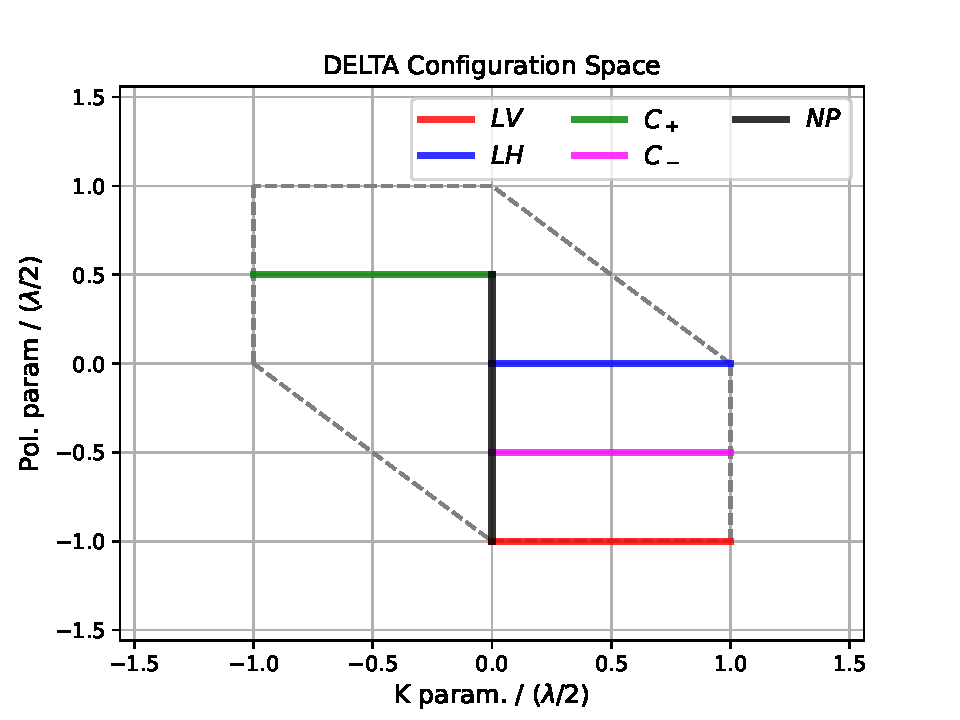
\includegraphics[width=.8\columnwidth]{config_space.pdf}
   \caption{Configuration space of DELTA 52}
   \label{fig:config_space}
\end{figure}

\section{Effects on orbit}

As previously stated, to address the residual field integrals of the ID, two corrector coils positioned adjacent to the ID operate within a feedforward system operating at a frequency of $\SI{10}{Hz}$. Figure \ref{fig:orbit_slow} illustrates the root mean square (r.m.s) of orbit distortions across all beam position monitors (bpms) for various ID configurations.

The first step in calculating the feedforward table involved filtering the measured orbit using the Slow Orbit Feedback System (SOFB), aiming to mitigate orbit drifts originating from other sources of perturbations. This process entailed determining the kicks of the SOFB correctors that most effectively accounted for the orbit distortions. Subsequently, all correctors, except for the two nearest to the ID, were reset to zero. Then, the orbit distortions generated by the ID can be approximated using the following equation.

\begin{equation}
    \Delta\Vec{x}_{ID} = M_{SOFB}\Delta\Vec{\theta}_{loc}
\end{equation}

Here, $M_{SOFB}$ represents the Jacobian matrix of the SOFB, and $\Delta\Vec{\theta}_{loc}$ denotes the kicks of the SOFB correctors. Subsequently, the filtered orbit was utilized in the Jacobian of the local correctors. It's important to note that all Jacobians were computed solely based on the storage ring model. The final stage involved interpolating the kicks for all permissible configurations, achieved through a 2D Gaussian model [cite Gaussian model].

The residual orbit distortion was quantified for all configurations with the  ID in a static position by implementing the feedforward correction method. As depicted in Figure \ref{fig:orbit_slow},  the resulting orbit residue measures less than $\SI{2}{\mu m}$.

\begin{figure}[!h]
    \centering
   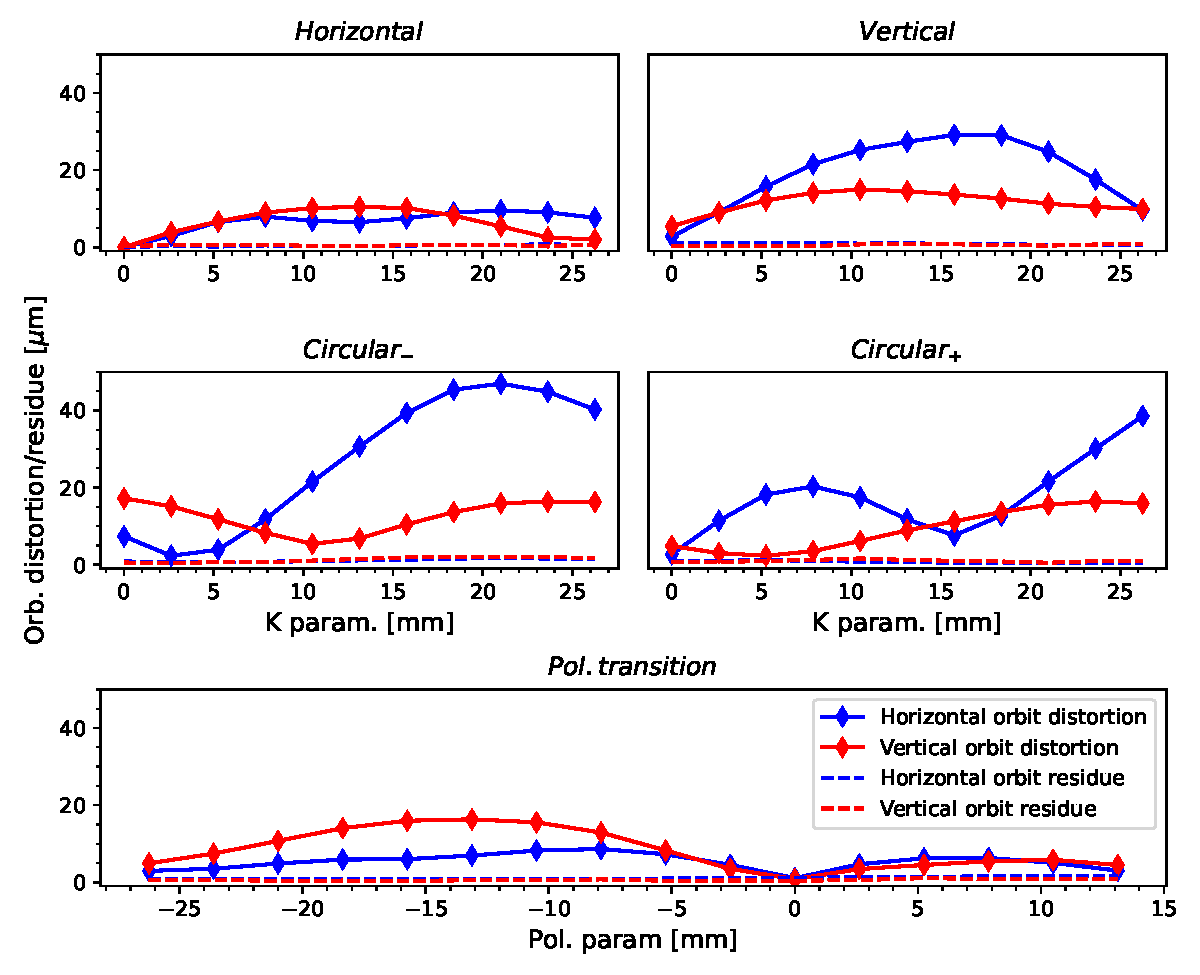
\includegraphics[width=\columnwidth]{THPS18_f2.pdf}
   \caption{Effects of DELTA 52 on orbit and residue of feedforward correction for all DELTA configurations}
   \label{fig:orbit_slow}
\end{figure}

In addition to statically characterizing orbit distortion and residual effects from feedforward compensation, the dynamic impact of device motion was assessed. An example of significant orbit distortion occurred during circular polarization with negative K parameter variations ranging from $\SI{0}{mm}$ to $\SI{13.125}{mm}$, moving at a maximum speed of 1 mm/s. Figure \ref{fig:orbit_fast} displays the r.m.s of the orbit distortion across all bpms. The figure illustrates that feedforward compensation effectively mitigates dynamic distortions from ID movement.

\begin{figure}[!h]
    \centering
   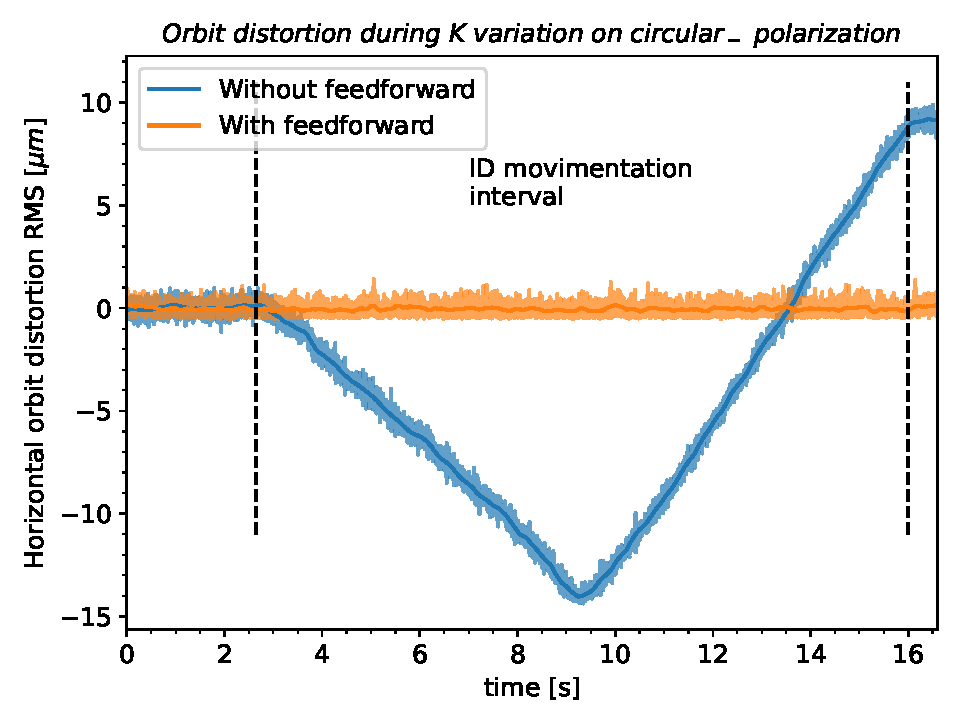
\includegraphics[width=0.8\columnwidth]{THPS18_f4.pdf}
   \caption{Effects ID movimentation on orbit and feedforward compensation.}
   \label{fig:orbit_fast}
\end{figure}

\section{Effects on optics}
\subsection{Linear optics}

The effects of the ID in the linear optics were also measured despite being very small. The tune shifts as a function of the device configuration can be seen in Figure \ref{fig:tunes}, where it is observed a tune shift of only 0.0012 in the worst-case.

\begin{figure}[!h]
    \centering
   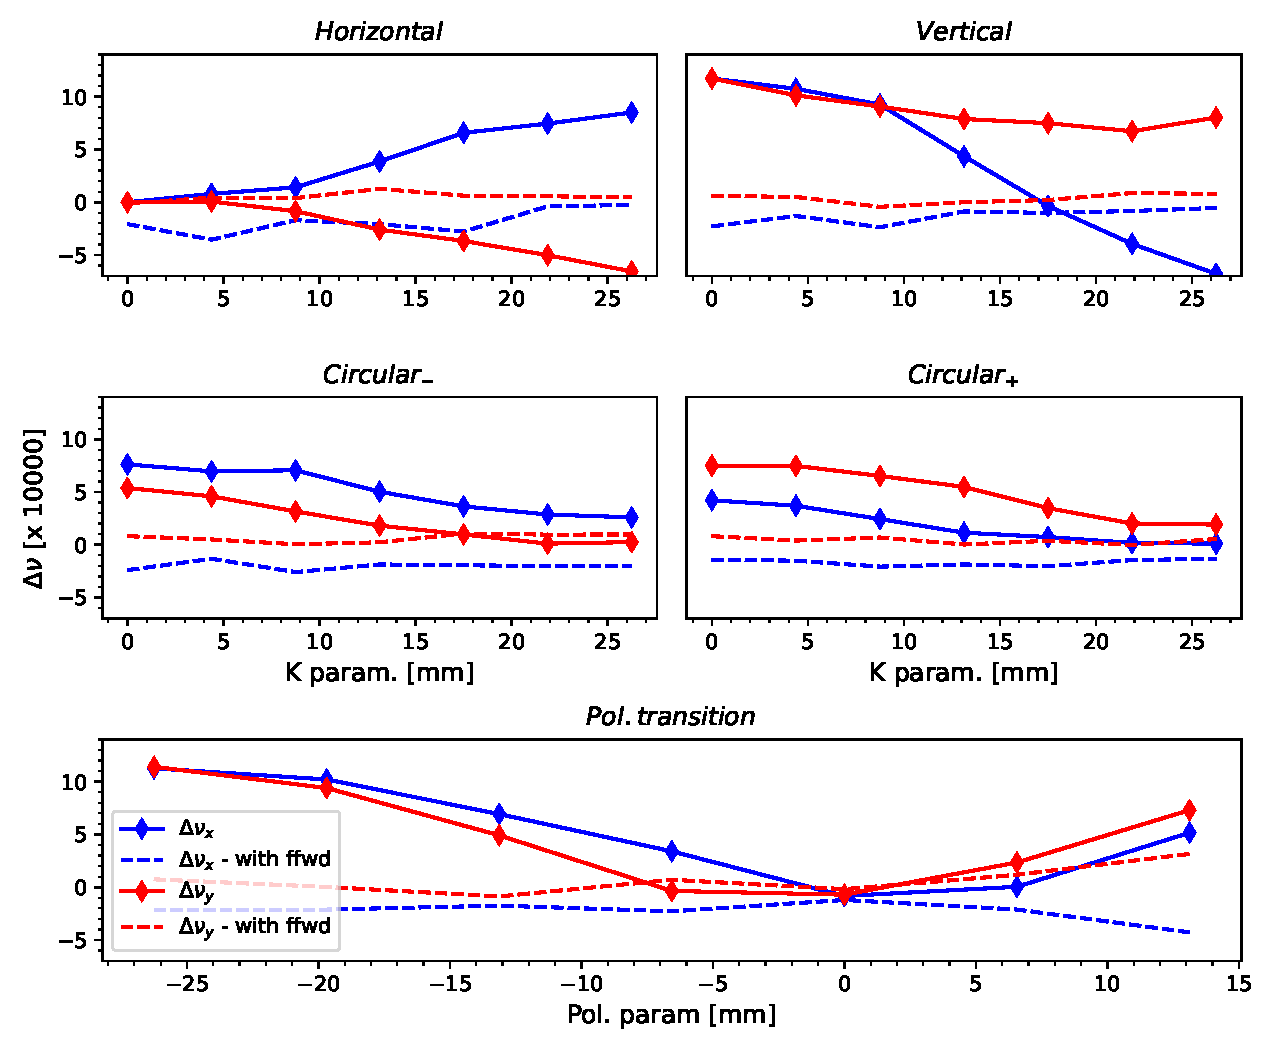
\includegraphics[width=\columnwidth]{THPS18_f3.pdf}
   \caption{Effects of DELTA 52 on tunes}
   \label{fig:tunes}
\end{figure}

Two methods have been employed to counteract these influences on linear optics. The initial approach involves determining the orbit response matrix of the system for each DELTA configuration and subsequently minimizing the variance between the matrix in the standard setup (K=0, horizontal polarization) and all alternative configurations by adjusting the normal quadrupole strengths of the ID section. Nevertheless, owing to the marginal impact of the ID on optics, this technique proved ineffective, as the disparity in matrices resulting from various ID configurations equaled the resolution of matrix measurements.

The alternative method only addresses tune shifts by utilizing the two quadrupole triplets immediately preceding and following the ID's straight section. In this approach, the Jacobian describing the influence of quadrupole strengths on the tunes was computed based on empirical measurements. As the quadrupoles are adjusted symmetrically, this Jacobian forms a $2 \times 3$ matrix. The efficacy of this correction method is illustrated in Figure \ref{fig:tunes}, indicating that the tune shifts are constrained within a variation range of less than 0.0004. It's noteworthy that the adjustments made to the quadrupole strengths were below $0.07\%$.

The final adjustment in linear optics focused on correcting coupling. This correction method mirrored the initial approach tested for uncoupled optics. However, in this case, the objective was to minimize differences in the off-diagonal terms of the orbit response matrix relative to the matrix in the standard setup. This was achieved by adjusting the strength of the adjacent skew quadrupoles. For a non-invasive coupling estimation, the measured Orbit Response Matrices (ORMs) were utilized as inputs for the LOCO algorithm \cite{Safranek} to calibrate the storage ring model. Subsequently, employing this model, the merit figure used to estimate the coupling was the minimum tune separation. Figure \ref{fig:coupling} illustrates the difference in coupling with and without the activation of skew feedforward. It's evident that feedforward implementation mitigates coupling variation across the K parameters. Similar to the feedforward for corrections, a Gaussian model was employed to interpolate skew strengths for all possible configurations.
 
\begin{figure}[!h]
    \centering
   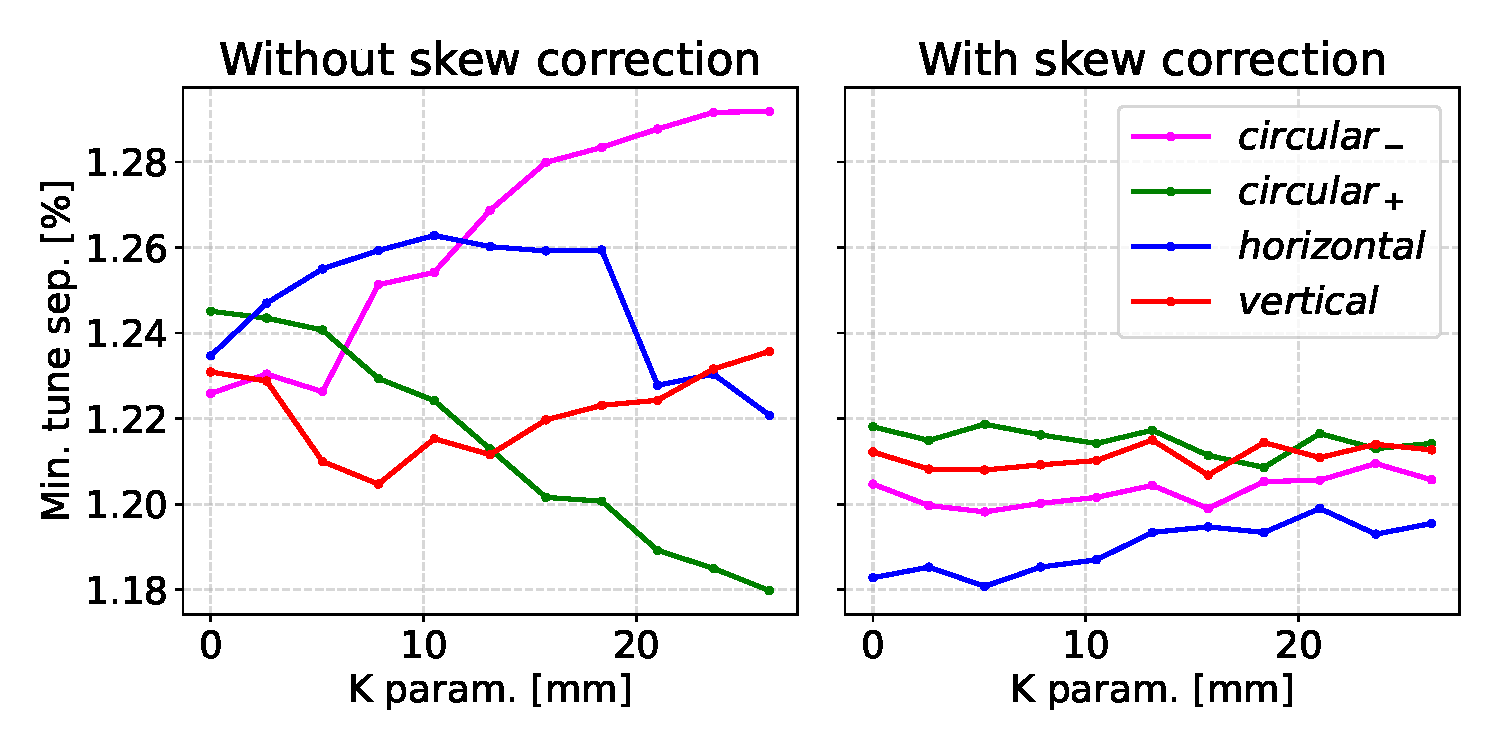
\includegraphics[width=\columnwidth]{coupling.pdf}
   \caption{Effects of DELTA 52 on coupling}
   \label{fig:coupling}
\end{figure}


\section{Dynamic aperture}

Following the DELTA installation, no impact was noted on the injection efficiency. This observation aligns with findings from tracking simulations on machines with random errors. These simulations were executed using Trackcpp \cite{Trackcpp}, where the measured ID fields were modeled as kickmaps. Dynamic aperture (DA) calculations were performed for each ID configuration across 20 machines with random errors. The results of these calculations are shown in Figure \ref{fig:dynapt}.


\begin{figure}[!h]
    \centering
   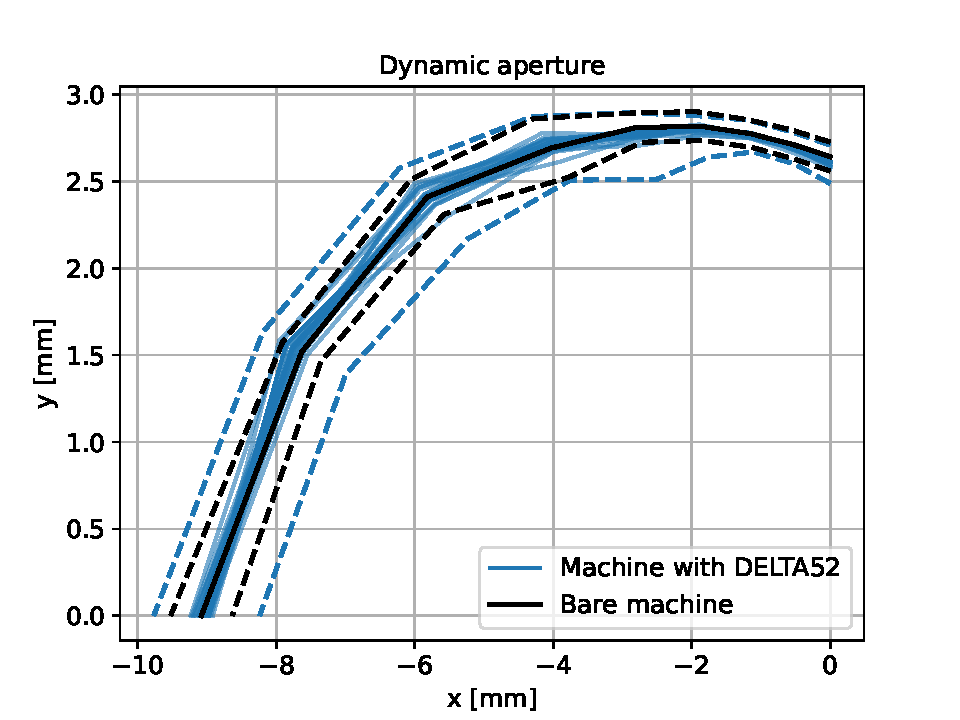
\includegraphics[width=0.95\columnwidth]{dynapt.pdf}
   \caption{Impact of DELTA 52 on dynamic aperture: Solid lines depict the average  DA across the 20 machines, whereas dashed lines illustrate the r.m.s of the DA.}
   \label{fig:dynapt}
\end{figure}

\section{Equilibrium parameters}
The influence on beam emittance and energy spread resulting from the inclusion of the ID was calculated utilizing analytical expressions derived from synchrotron radiation integrals \cite{Lee:1999}.

\begin{figure}[!h]
    \centering
   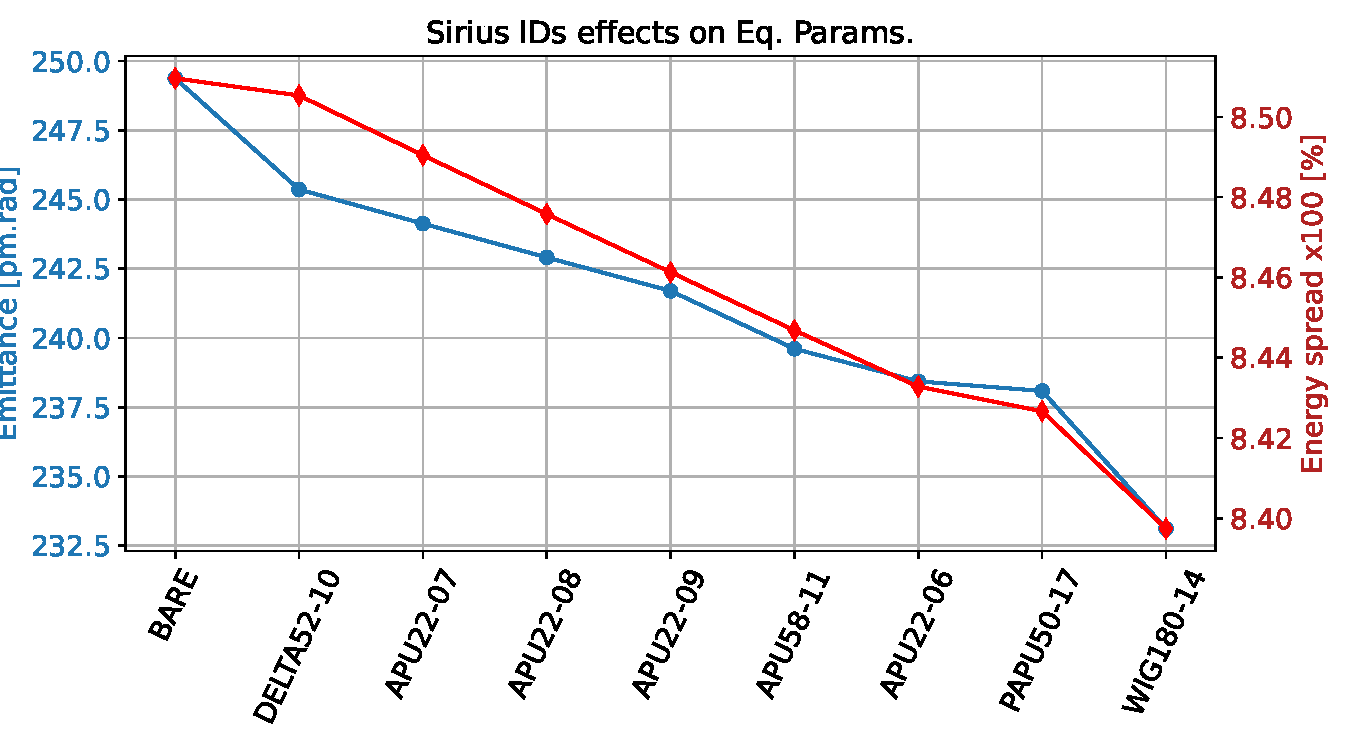
\includegraphics[width=\columnwidth]{eqparams.pdf}
   \caption{Effects SIRIUS IDs on equilibrium parameters.}
   \label{fig:eq_param}
\end{figure}

\section{CONCLUSIONS}


\section{ACKNOWLEDGEMENTS}


	\begin{thebibliography}{14} % Use for 1-9 references

    %\cite{Liu:IPAC23-WEOGA2}
\bibitem{Liu:IPAC23-WEOGA2}
   L. Liu \emph{et al.},
   \textquotedblleft{Status of SIRIUS operation with users}\textquotedblright,
   presented at the IPAC’23, Venice, Italy, May 2023, paper WEOGA2, this conference.   
    
    % \bibitem{Wiedemann:2015}
    %     Wiedemann, Helmut,
    %     \textquotedblleft{Overview of Synchrotron Radiation}\textquotedblright,
    %     in \emph{Particle Accelerator Physics}, Berlin Heidelberg, Germany: Springer, 2007, pp. 749-788.


    \bibitem{Beamlines}
        LNLS,
        \textquotedblleft{SIRIUS Beamlines}\textquotedblright,
        available at https://lnls.cnpem.br/beamlines/

    \bibitem{Vilela:IPAC17-WEPIK053}
        L. N. P. Vilela \emph{et al.},
        \textquotedblleft{Studies of DELTA-Type Undulators for Sirius}\textquotedblright,
        in \emph{Proc. IPAC’17}, Copenhagen, Denmark, May 2017, pp. 3045--3047.
        \url{doi:10.18429/JACoW-IPAC2017-WEPIK053} 
    
    %\cite{Vilela:IPAC18-TUPMK003}
    \bibitem{Vilela:IPAC18-TUPMK003}
   L. N. P. Vilela, R. Basilio, J. F. Citadini, J. R. Furaer, and F. Rodrigues,
   \textquotedblleft{Advances in the Sirius DELTA-Type Undulator Project}\textquotedblright,
   in \emph{Proc. IPAC’18}, Vancouver, Canada, Apr.-May 2018, pp. 1491--1493.
   \url{doi:10.18429/JACoW-IPAC2018-TUPMK003}  

    %\cite{Ascenção:IPAC23-MOPM088}
\bibitem{Ascenção:IPAC23-MOPM088}
   G. Ascenção, M. Alves, L. Liu, and X. Resende,
   \textquotedblleft{Study of insertion devices effects in SIRIUS}\textquotedblright,
   in \emph{Proc. IPAC’23}, Venice, Italy, May 2023, pp. 1184--1187.
   \url{doi:10.18429/JACoW-IPAC2023-MOPM088}    

\bibitem{Safranek}
	 J. Safranek,
		\textquotedblleft{Experimental determination of storage ring optics using orbit response measurements}\textquotedblright,
		\emph{Nucl.  Instr. Meth. A}, vol 388, pp.27--36, 1997.
        \url{doi:10.1016/S0168-9002(97)00309-4}

    \bibitem{Trackcpp}
        LNLS Accelerator Physics Group,
        \textquotedblleft{Tracking library}\textquotedblright,
        available at https://github.com/lnls-fac/trackcpp
        


        \bibitem{Lee:1999}
        S. Y.Lee,
        \textquotedblleft{Physics of Electron Storage Rings}\textquotedblright,
        in \emph{Accelerator physics}, London, UK: World Scientific, 1999, pp. 383-458.


           


%    \bibitem{Liu:2015jpo}
%        L. Liu, N. Milas, A. Mukai, X. Resende and F. de Sá,
%        \textquotedblleft{Upgraded Optics for Sirius With Improved Matching of Electron and Photon Beam Emittances}
%        \url{doi:10.18429/JACoW-IPAC2015-TUPWA007}
        
%    \bibitem{Liu:IPAC2016-THPMR011}
%        L. Liu, X.R. Resende, A.R.D. Rodrigues, F. H. de Sá,
%       \textquotedblleft{{I}njection {D}ynamics for {S}irius {U}sing a {N}onlinear {K}icker}\textquotedblright,
%       in \emph{Proc. IPAC’16}, Busan, Korea, May 2016, pp. 3406--3408.
%       \url{doi:10.18429/JACoW-IPAC2016-THPMR011} 
 
%    \bibitem{deSá:IPAC2016-THPMR012}
%        F. H. de Sá, L. Liu, X.R. Resende,
%       \textquotedblleft{{O}ptimization of {N}onlinear {D}ynamics for {S}irius}\textquotedblright,
%       in \emph{Proc. IPAC’16}, Busan, Korea, May 2016, pp. 3409--3412.
%       \url{doi:10.18429/JACoW-IPAC2016-THPMR012}       
       
%	\bibitem{Huang:2013}
%		X. Huang, J. Corbett, J. Safranek, J. Wu,
%		\textquotedblleft{An algorithm for online optimization of accelerators}\textquotedblright,
%		\emph{Nucl.  Instr. Meth.}, vol 726, pp. 77--83, 2013.
%        \url{https://doi.org/10.1016/j.nima.2013.05.046} 

%    \bibitem{Huang:2015}
%		X. Huang, J. Safranek,
%		\textquotedblleft{Online optimization of storage ring nonlinear beam dynamics}\textquotedblright,
%		\emph{Phys. Rev. ST Accel. Beams}, vol 18, p. 18, .
%        \url{10.1103/PhysRevSTAB.18.084001} 
 
%    \bibitem{Liuzzo:IPAC2016-THPMR015}
%        S.M. Liuzzo, \emph{et al.},
%        \textquotedblleft{RCDS Optimizations for the ESRF Storage Ring}\textquotedblright,
%        in \emph{Proc. IPAC’16}, Busan, Korea, May 2016, pp. 3420--3423.
%       \url{doi:10.18429/JACoW-IPAC2016-THPMR015}   
    
%    \bibitem{Olsson:IPAC2018-WEPAL047}
%       D.K. Olsson,
%       \textquotedblleft{Online Optimisation of the MAX IV 3 GeV Ring Dynamic Aperture}\textquotedblright,
%       in \emph{Proc. IPAC'18}, Vancouver, BC, Canada, Apr. 4,, pp. 2281--2283,
%       \url{doi:10.18429/JACoW-IPAC2018-WEPAL047}

    
%    \bibitem{yang:ipac2022-tupopt064}
%        X. Yang,\emph{et al.},
%       \textquotedblleft{Online Optimization of NSLS-II Dynamic Aperture and Injection Transient}\textquotedblright,
%        in \emph{Proc. IPAC'22}, Bangkok, Thailand, Jun. 2022, pp. 1159--1162.

%       \url{doi:10.18429/JACoW-IPAC2022-TUPOPT064}
    
   
	\end{thebibliography}


\end{document}
